\documentclass{article} % For LaTeX2e
% We will use NIPS submission format
\usepackage{nips13submit_e,times}
% for hyperlinks
\usepackage{hyperref}
\usepackage{url}
% For figures
\usepackage{graphicx} 
\usepackage{subfigure} 
% math packages
\usepackage{amsmath}
\usepackage{amsfonts}
\usepackage{amsopn}
\usepackage{ifthen}
\usepackage{natbib}

\title{Project-I by Group MexicoCity}

\author{
Kevin Serrano\\EPFL\\
\texttt{kevin.serrano@epfl.ch} \And Youssef El Baba\\EPFL\\
\texttt{youssef.baba@epfl.ch} \And Alexandre Helfre\\EPFL\\
\texttt{alexandre.helfre@epfl.ch}
}

% The \author macro works with any number of authors. There are two commands
% used to separate the names and addresses of multiple authors: \And and \AND.
%
% Using \And between authors leaves it to \LaTeX{} to determine where to break
% the lines. Using \AND forces a linebreak at that point. So, if \LaTeX{}
% puts 3 of 4 authors names on the first line, and the last on the second
% line, try using \AND instead of \And before the third author name.

\nipsfinalcopy 

\begin{document}

\maketitle

\begin{abstract}
In this report, we discuss our implementation and findings for the project-I. We fit several methods to the regression dataset and compared them. We found that the input matrix is not ill conditioned and that ridge regression gives a better test error. Trying non-linear model doesn't help so the linear model is appropriate for this data set. We investigated some feature transformations. We also used a classification data set for which we found that the input matrix has full rank which means all inputs are correlated. We saw that the best test error can be achieved by computing the 0-1 loss using logistic regression.


\end{abstract}
\section{Five functions}
\begin{itemize}
\item \textit{leastSquaresGD(y,tX,alpha)} : Least squares using gradient descent, alpha is the step-size
\item \textit{leastSquares(y,tX)} : Least squares using normal equations
\item \textit{ridgeRegression(y,tX,lambda)} : Ridge regression using normal equations, lambda is the regularization coefficient
\item \textit{logisticRegression(y,tX,alpha)} : Logistic regression using gradient descent or Newton's method
\item \textit{penLogisticRegression(y,tX,alpha,lambda)} : Penalized logistic regression 

\end{itemize}
These functions are different machine learning methods.


\section{Data observation}
\label{sec:datadescr}
We have two data set. One for regression and one for classification. \begin{description}
\item[Regression] Consists of output variables $\mathbf{y}$ and input variables $\mathbf{X}$. The number of examples is $N = 1400$ and each input $\mathbf{x_n}$ has dimensionality $D = 48$. The first $34$ are real valued and the last $14$ are categorical, included $5$ that are binaries.
\item[Classification] Consists of output variables $\mathbf{y}$ and input variables $\mathbf{X}$. The number of examples is $N = 1500$ and each input $\mathbf{x_n}$ has dimensionality $D = 35$. 

\end{description}

\section{Regression}
Note that all the gradient descent methods used the eps threshold (machine dependant) in Matlab in the gradient descent function, to allow for a maximum number of iterations. This might make the gradient descent process slow though, so feel free to set another number if needed. We changed it later to 1/1000, so the numbers for the test Errors might be different depending on this parameter when you run the code (the global trends are the same though), since the number of iterations will be different.
\subsection{Data visualization and cleaning}
Most variables are normally distributed with various means. The first 34 input variables are Gaussian and the last 14 are categorical. The boxplot in Figure \ref{fig:boxplot} shows us that the data is not centred. Given that, we normalized and centred the first 34 variables and let the others untouched. Plotting the histogram of $\mathbf{y}$ as shown if Figure \ref{fig:outputhist} showed us that the data is compact and there is no outlier, but we can see a second bump.\\
For regression, $\mathbf{\tilde{X}}$ has rank 49, included the one vector, so no redundancy in variables.\\

To help us with the task of finding which transforms could be useful in better predicting the output from the given predictors, we decided to use the help of the Pearson linear correlation coefficient. This coefficient basically gives a number indicating the strength (in its absolute value) of a linear model fit between two variables. Obviously, we could visually inspect multiple scatter plots between each variable and the output, and also with the other variables, but this can (for obvious reasons) be somewhat of an overkill and could lead to subjective mistakes. The Pearson coefficient allows us to selectively choose which variables (and which possible transforms accordingly) could be used to fit a good model, in a very fast manner (simply adding columns to $\mathbf{\tilde{X}}$ and checking their correlation coefficients). The Spearman coefficient could also be used, but is much less adapted for linear fitting in our case.\\

We checked the correlation between output and input variables. The correlation matrix helped us to discover which variables where correlated to no other variables nor the output. We could remove these variables. We used the Pearson correlation. The variables that are neither significantly correlated with the output, nor with the other input variables, were found and were later removed from our model for simplicity and to improve generalization performance.
\begin{figure}
\centering
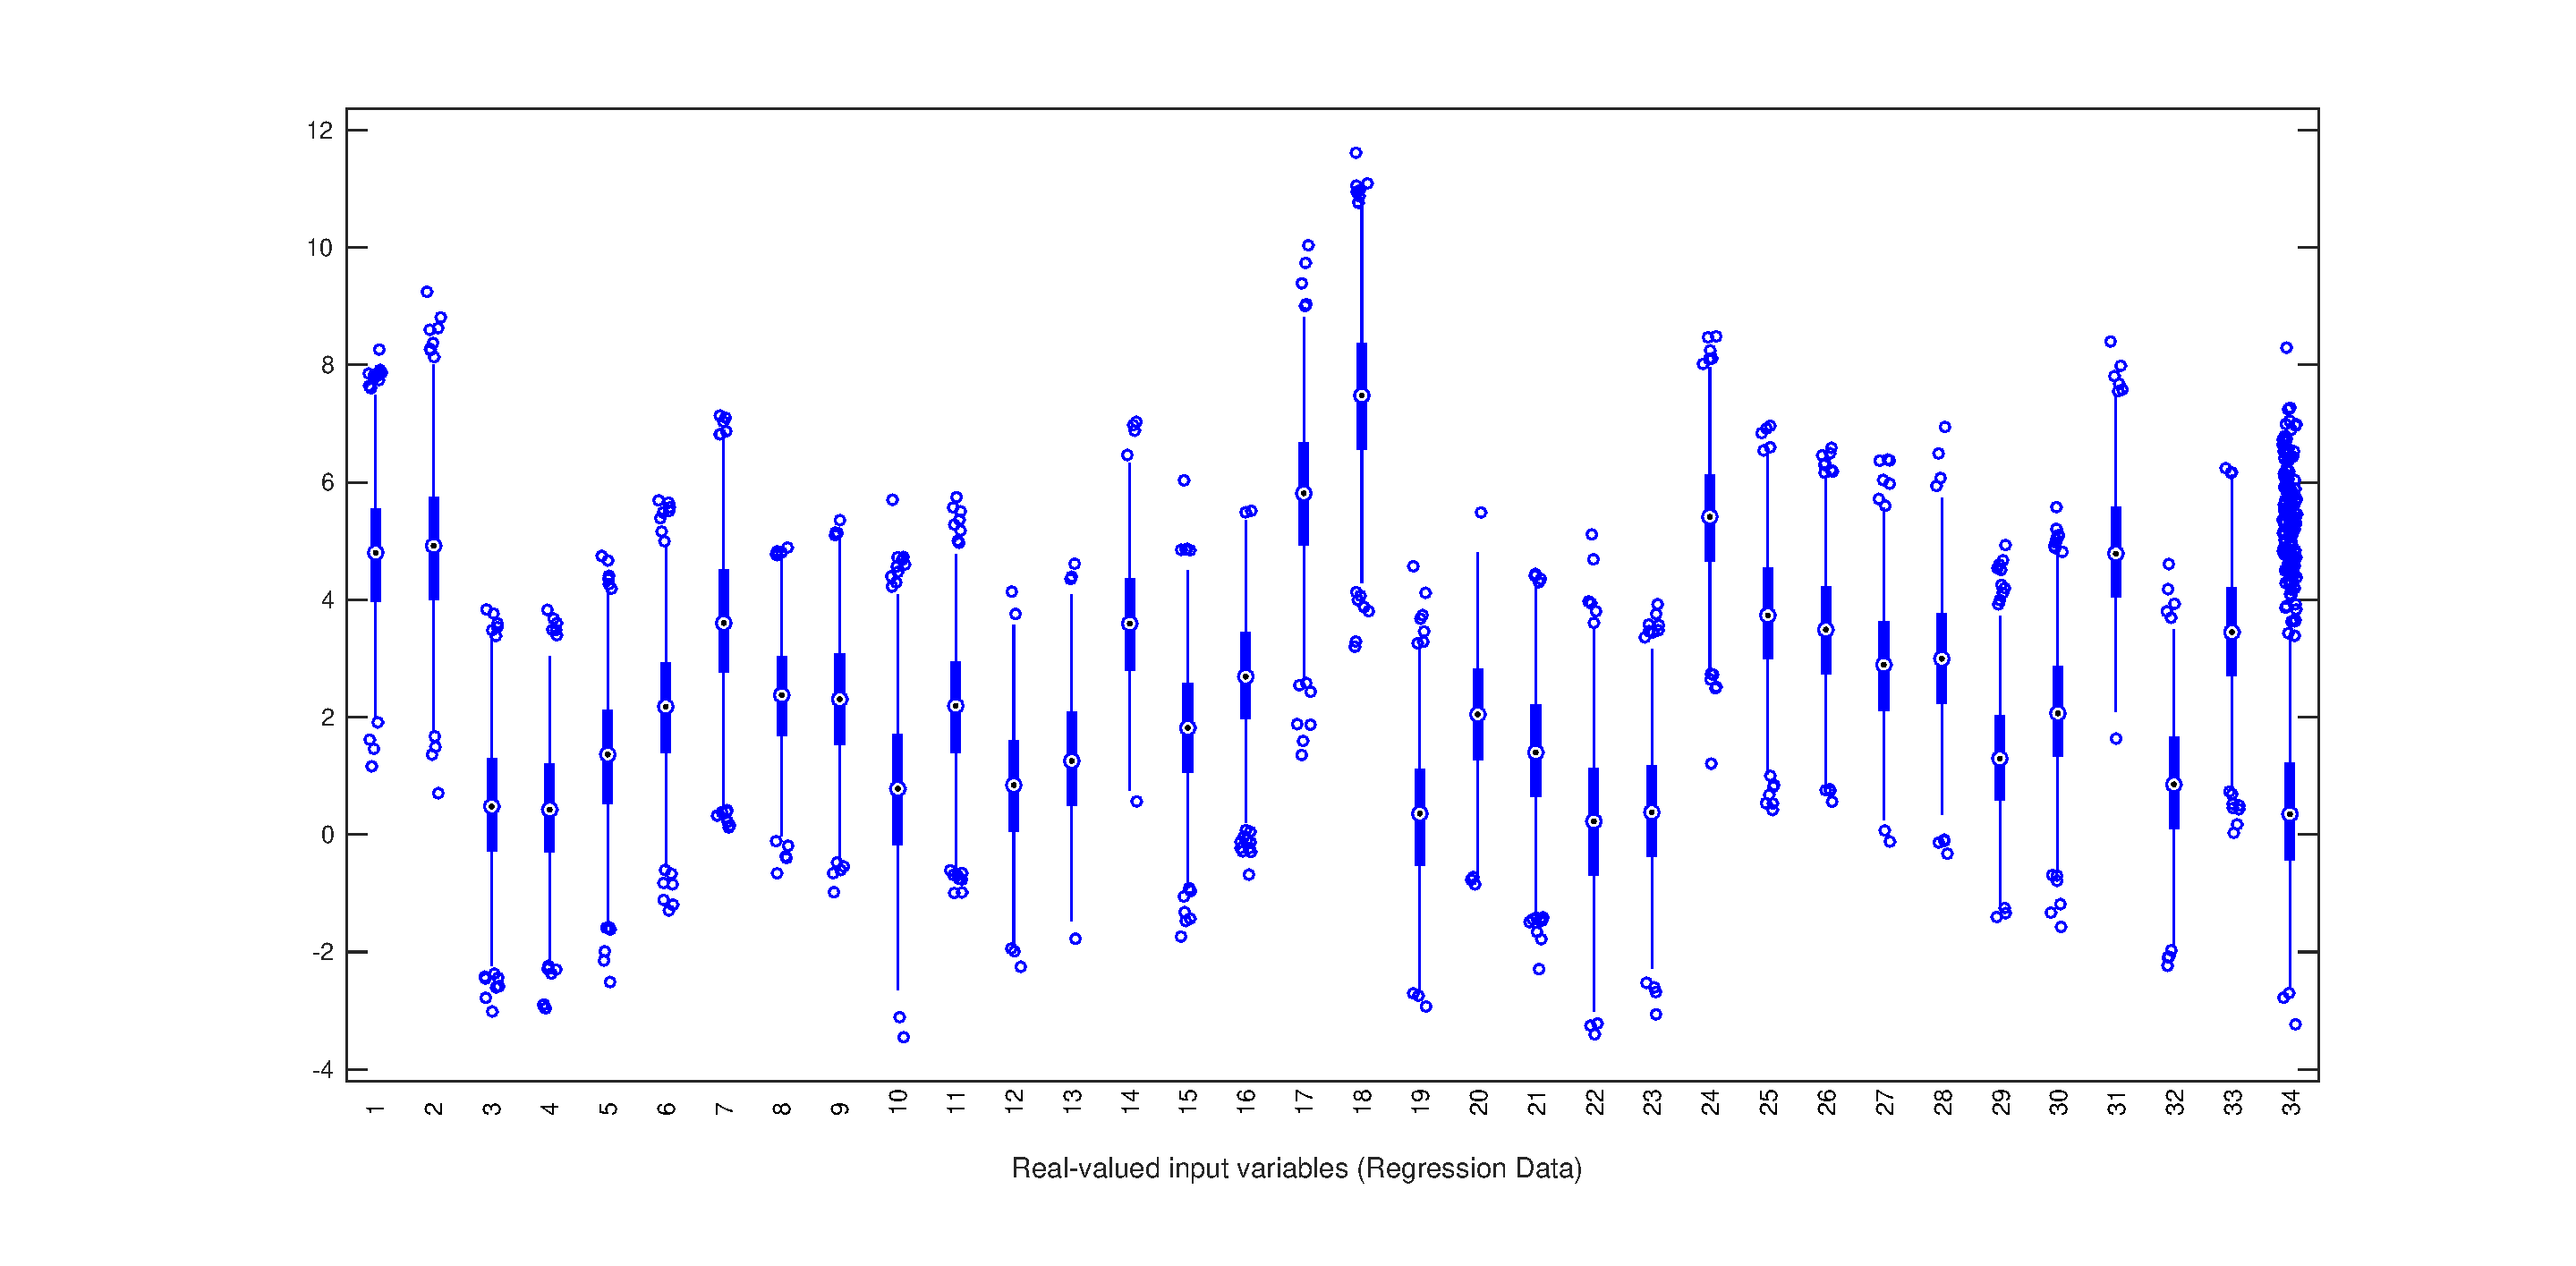
\includegraphics[width=0.7\textwidth]{images/boxplot_xtrain_reg.eps}
\caption{Boxplot of all input variables for regression (except categorical)}
\label{fig:boxplot}
\end{figure}

\begin{figure}
\centering
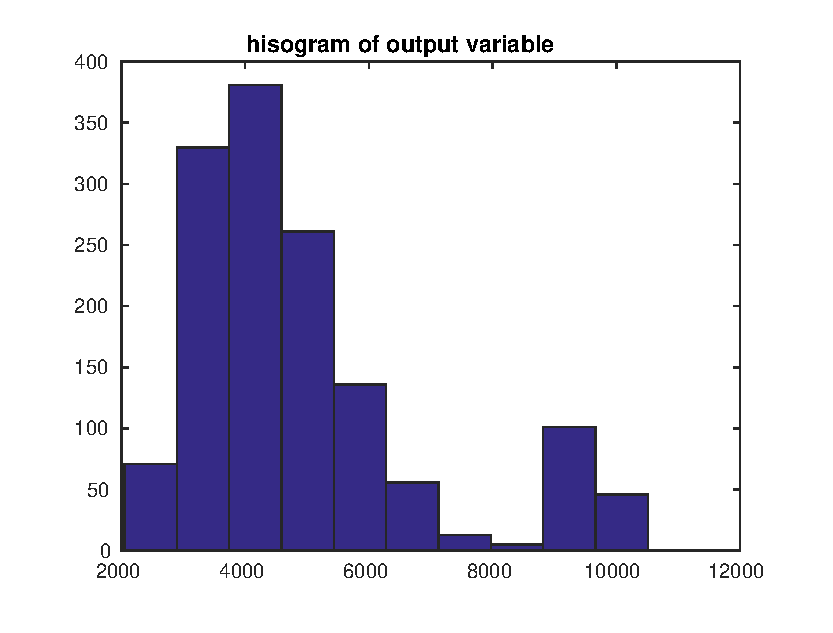
\includegraphics[width=0.45\textwidth]{images/hist_output.eps}
\caption{Histogram of output variable $\mathbf{y}$}
\label{fig:outputhist}
\end{figure}

\subsection{Least Squares}

The mean gives a RMSE of 0.99964, over normalized $\mathbf{y}$.

Applying the least squares method on the data without cleaning yields a training RMSE of $0.48244$. Given that, we see that the RMSE is cut by half so the input data are meaningful.


We got the RMSE down to train error 0.3605 (with estimated test error 0.3805) using direct least squares, simply by adding the squares of the 18th and 34th variables. When we added the squares of all the variables, we only got a train error of 0.3405 but this is clearly overfit because the corresponding test error estimate is 0.3765.

We tested taking the squares of the 18th and the 34th variable individually and a curious thing happened: when we removed the 18th variable (squared) the test error increased to to 0.3881, but when we removed the 34th variable (squared) the test error increased much more significantly to 0.4987.
\label{sec:regridgreg}
By visually inspecting the Pearson correlation graphs, a good strategy to spot well correlated input variables was to take the intersection of the two methods (we’re only considering ). To do that, we tried multiplying the two coefficients (for each variable) and taking the mean. Both strategies clearly showed the 18th and 34th variables are best correlated. We can limit our variable transform to these two (we only have 1400 data points, so with a dimension 48 we’re already lacking data, by introducing spurious transforms we would be adding fuel to the fire and causing overfitting.)

\subsection{Ridge Regression}
After applying least squares, we have also done a cross validation using seeds. The result is shown in Figure \ref{fig:ridreggcv}.
\begin{figure}
\centering
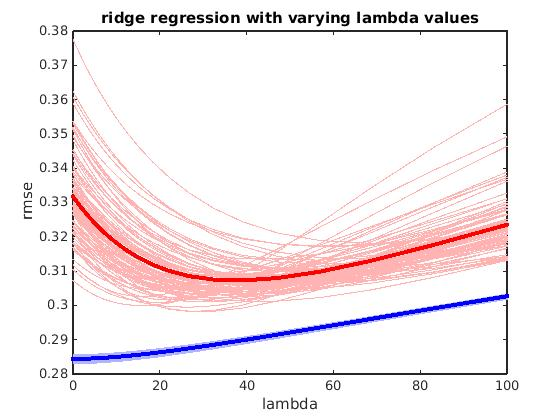
\includegraphics[width=0.5\textwidth]{images/ridgeRegCV.jpg}
\caption{Cross validation : Ridge regression with different lambda values }
\label{fig:ridreggcv}
\end{figure}
We realized that the RMSE decreased for a parameter $\lambda = 39.0694$ to a RMSE of $0.3073$. We can see that on the Figure \ref{fig:ridreggcv}.

\subsection{Feature transformations}
We tried dummy variables for all regression categorical ones. We could only find a significant linear correlation (using Spearman) for the 2nd class of the variable 44, 2nd and 4th class of the 47th.

We tried keeping the polynomial transforms and removed all categorical variables. The test error went down to 0.33043.\\

Adding back the mentioned dummy variables 44 and 47 actually increased the test error to 0.33105. This leads the matrix $\mathbf{\tilde{X}}$ to become ill conditioned.

We also tried adding square root of the 18th and 34th variable, that means $\sqrt{|X_{n18}|}$ and $\sqrt{|X_{n34}|}$ of $\mathbf{X}$. With the 18th the test error went up to 0.32137 and with the 34th it went up to 0.39349. So this doesn't help and we decided not tu use square root transformation.

We decided to ignore all the un-correlated variables for regression, giving a test error of 0.33173 while including the significant transformations of the 18th and 34th variables discussed before. We decided to opt for a simpler model because of Occam’s Razor.

By isolating the 18th and 34th input variables, and producing polynomial transforms of them using the myPoly function, and then measuring their Pearson correlation coefficient with the output, we could see that the cube and the power 5 of the 18th variable, and powers up to 6 for the 34th variable are correlated with the output. When adding these feature transformations, we could lower the test error to 0.3307, which is quite lower now than the starting test error of 0.3805.
\section{Classification}
\subsection{visualization and cleaning}

For classification, the rank of $\mathbf{\tilde{X}}$ is 35 plus the one vector. Given the data description from section \ref{sec:datadescr}, this tells us that $\mathbf{\tilde{X}}$ is not ill-conditioned.\\ The range of $\mathbf{y}$ is between $-1$ and $1$. We also modified the values $-1$ from $\mathbf{y}$ to 0 to be consistent with the book of Murphy. We show the boxplot for $\mathbf{X}$ in Figure \ref{fig:boxplotclass}.
\begin{figure}
\centering
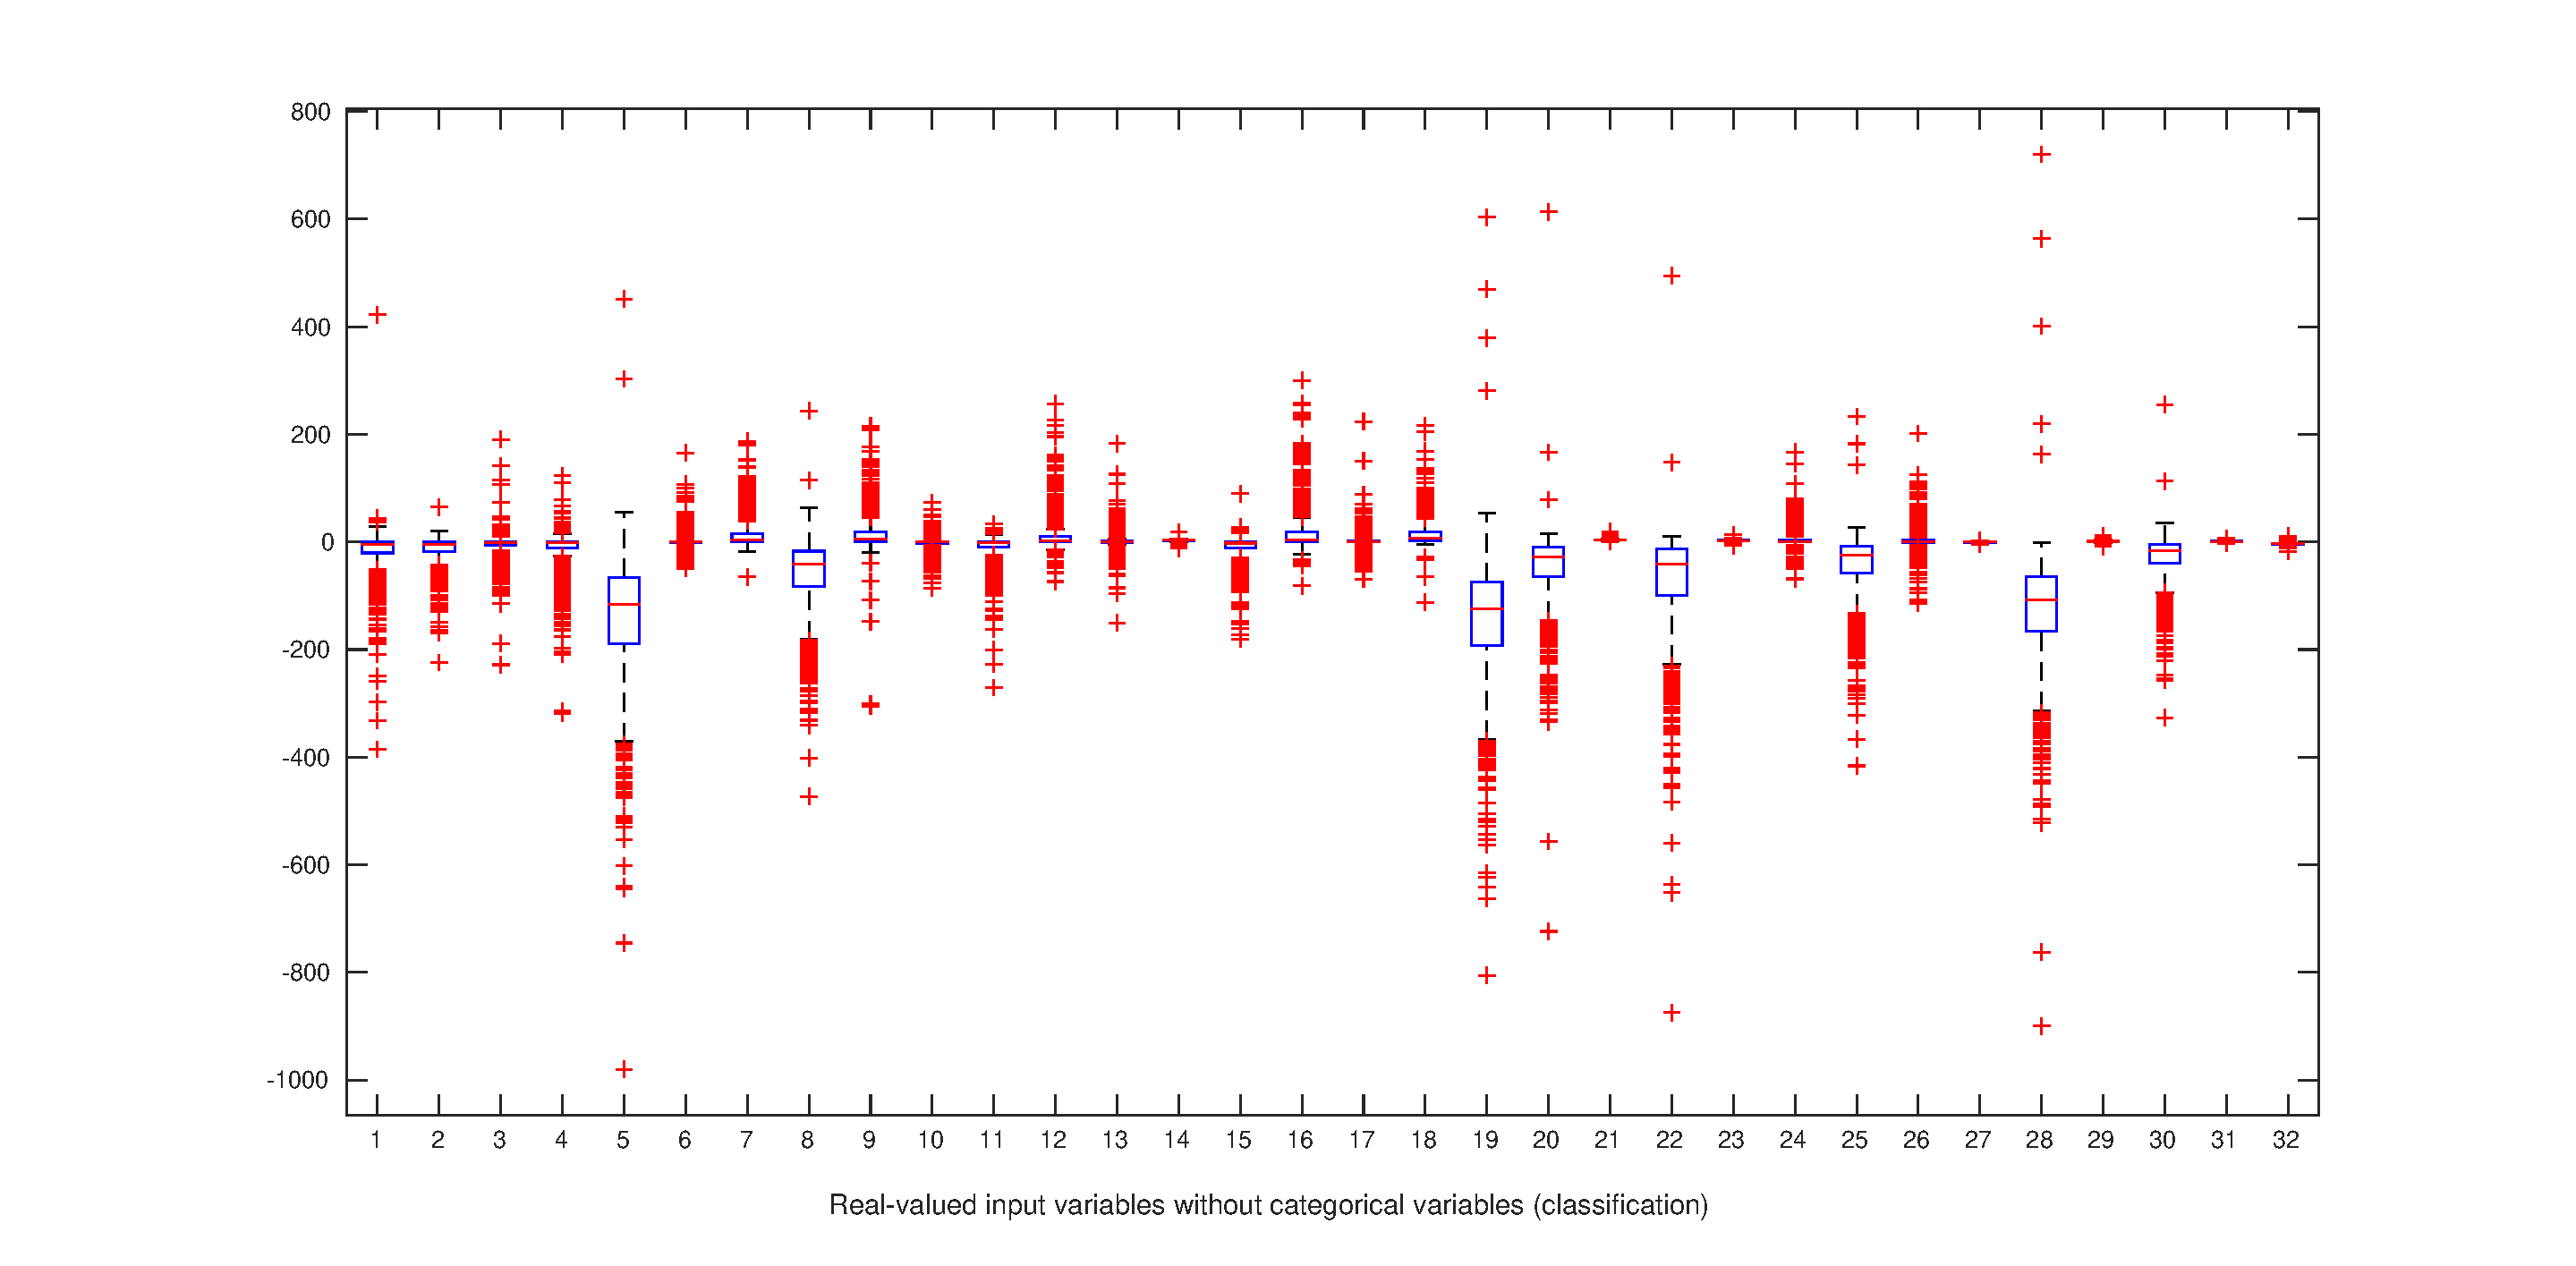
\includegraphics[width=0.8\textwidth]{images/boxplot_class.eps}
\caption{Boxplot for input variable $\mathbf{X}$ for classification}
\label{fig:boxplotclass}
\end{figure}
\subsection{Logistic Regression}
For the classification, we repeated the procedure describe in section \ref{sec:regridgreg}. We found that the 11th and the 24th variables are best correlated with the output, therefore we used feature transforms on those as described in section \ref{sec:ftransclass}.
\subsection{Feature transformations}
\label{sec:ftransclass}
We tried to use simple logistic regression using all the variables, the estimated RMSE test error was 0.27099. Also we tried using square root on the 11th and 24th variables which actually improved our test error to 0.26779. We can also use squares of the variables instead of the square root. Applying this alone the test error decreased to 0.26715. Adding both transformations got us a decrease to a test error of 0.26474. We also tried to remove all categorical variables as we did in regression, but the test error increased to 0.3396, so their information was needed and cannot be ignored.

We then found that, since Pearson correlation predicted better correlation of square roots than squares but squares were actually better able to decrease test error, it might be a good idea to include 3rd degree transforms of the 11th and 24th variables for logistic regression. After having added them, the test error increased to 0.26656. Thus taking higher orders doesn’t seem to help. We then tried to include a dummy variable transform, but that increased the test error significantly to 0.32625, therefore we’re not going to use them.
\subsection{Penalized logistic regression}
We could improve the test error by cross-validation. The Figure \ref{fig:crossval} shows the three different tests error RMSE, 0-1 loss and log loss. We used different numbers of seeds to have a better prediction for our test error.
\begin{figure}
\centering
\subfigure[0-1 loss]{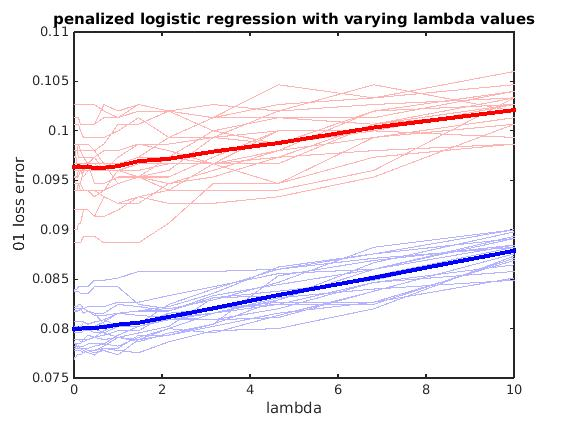
\includegraphics[width=0.6\textwidth]{images/penLogRegCrossVall01Loss.jpg}}
\subfigure[rmse]{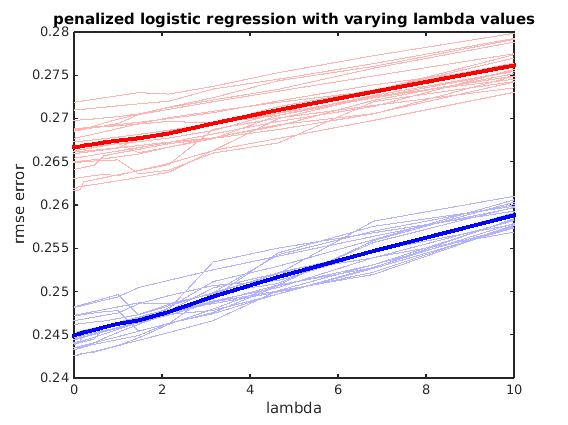
\includegraphics[width=0.6\textwidth]{images/penLogRegrmse.jpg}}
\subfigure[log loss]{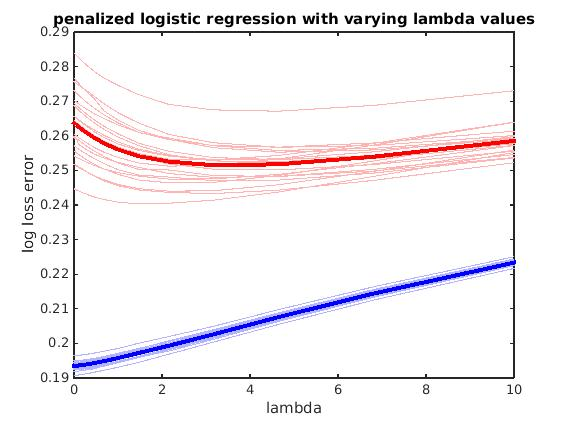
\includegraphics[width=0.6\textwidth]{images/penLogRegLogloss.jpg}}
\caption{Cross-validation : penalized logistic regression with different lambda values}
\label{fig:crossval}
\end{figure} 
\section{Summary}
As we have seen, the cross validation helps to have a better test error.\\
We obtained these RMSE for regression.
\begin{description}
\item[leastSquaresGD] We achieved a RMSE of 0.6852
\item[leastSquares] We achieved a RMSE of 0.3317
\item[RidgeRegression] We achieved a RMSE of 0.3073
\end{description}
For the regression, we saw that the best method was Ridge Regression. The best parameter was $\lambda =  39.0694$ and we achieved a test error of 0.3073.

For the classification, the best method was penalized logistic regression. We obtained different results depending the type of error we computed. \begin{description}
\item[RMSE] We achieved a test error of 0.2644.
\item[01 loss]We achieved a test error of 0.09486.
\item[log loss] We achieved a test error of 0.25149.
\end{description}
With logistic regression we obtained different results depending the type of error we computed. \begin{description}
\item[rmse] We achieved a test error of 0.2644.
\item[01 loss]We achieved a test error of 0.09486.
\item[log loss] We achieved a test error of 0.2637.
\end{description}
We see that there is only a small improvement with the log loss error with penalized logistic regression.
The best error we achieved is through the penalized logistic regression method and using the 0-1 loss error.

\subsubsection*{Acknowledgments}
We would like to thanks the teaching team for their availability during the exercise session but also on the forum. We also want to thanks Youssef who organized the milestone of the project.

\subsubsection*{References}
Kevin Murphy, Machine Learning : A Probabilistic Perspective {\em The MIT Press
Cambridge, Massachusetts
London, England,2012} 


\end{document}
